\documentclass[aspectratio=169]{beamer}

\usepackage{xcolor}
\usepackage{graphicx}
\usepackage{multimedia}
\usepackage[T1]{fontenc}
\usepackage{lmodern}
\usepackage{tikz}
\usetikzlibrary{positioning,calc,shadings,shapes.geometric,arrows.meta,fit,backgrounds}

\title{Stash House}
\subtitle{Reconstituting Disciplined Secret Use under Local Disorder}
\author{Franklin Diaz}
\institute{University of Colorado}
\date{March 2026}
% --- Custom Styling ---
\tikzset{section number/.style={inner sep=0pt,draw=none},
section/.style={inner sep=0pt,draw=none,text=blue,align=center},
subsection/.style={inner sep=0pt,draw=none,text=gray,align=center}
}

\makeatletter
\def\sectionsubtitle#1{\gdef\@sectionsubtitle{#1}}
\AtBeginSection[]{
\begingroup
\setbeamercolor{background canvas}{bg=gray!30}
\begin{frame}
\begin{tikzpicture}[remember picture,overlay]
\coordinate[yshift=-10mm] (rectsouthwest) at (current page.north west);
\coordinate[yshift=-10mm] (rectsoutheast) at (current page.north east);
\fill[white] (current page.north west) rectangle (rectsoutheast);
\shade [left color=gray,right color=white] (rectsouthwest) rectangle +(\paperwidth,-0.02);
\node[section,anchor=center] at (current page.center) (title) {\fontsize{20}{20}\selectfont\insertsectionhead};
\node[subsection,below=5mm of title]  (subtitle) {\@sectionsubtitle};
\end{tikzpicture}
\end{frame}
\gdef\@sectionsubtitle{}
\endgroup
}
\makeatother

\begin{document}

{
\usebackgroundtemplate{
\includegraphics[width=\paperwidth]{../../static/images/technology-presentation.jpg}}
\begin{frame}
\titlepage
\note[item]{The modern developer workstation is characterized by high entropy. We aren't just building a vault; we're recovering
stewardship.}
\end{frame}
}

{
\usebackgroundtemplate{
\includegraphics[width=\paperwidth]{../../static/images/section.jpg}}
\sectionsubtitle{\textcolor{black}{From Chaos to Stewardship}}
\section{The Problem: Local Disorder}
}

{
\usebackgroundtemplate{
\includegraphics[width=\paperwidth]{../../static/images/tech-white.jpg}}
\begin{frame}
\frametitle{Admitting the Entropy Problem}
\begin{columns}
\column{0.5\textwidth}
\begin{itemize}
\item \textbf{Credential Sprawl:} Cloud tokens, SSH keys, and DB credentials in history files and unencrypted artifacts.
\item \textbf{Passive vs. Active:} Detection (GitGuardian/Gitleaks) is not remediation.
\item \textbf{The Goal:} Reconstitute discipline without destroying developer velocity.
\end{itemize}
\column{0.5\textwidth}
\begin{figure}
\centering

\includegraphics[width=0.77\textwidth]{../../static/images/problem.jpg}
\caption{\textcolor{black}{The state of local disorder.}}
\end{figure}
\end{columns}
\end{frame}
}

\begin{frame}
\frametitle{System Architecture}
\centering
\resizebox{0.8\textwidth}{!}{
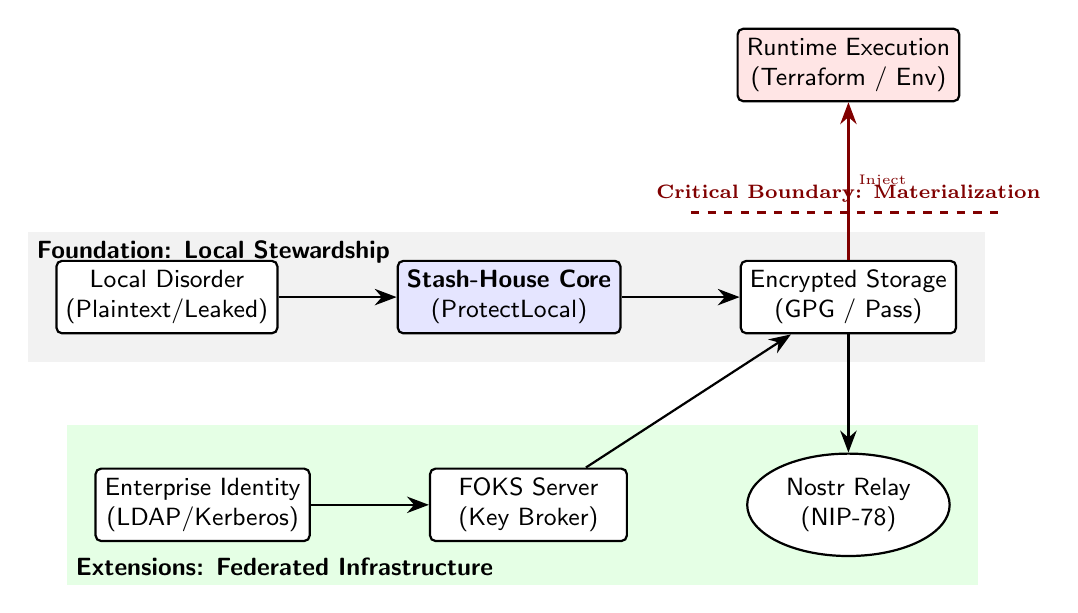
\begin{tikzpicture}[
node distance=1.2cm and 1.5cm,
font=\sffamily\small,
box/.style={rectangle, draw, thick, fill=white, minimum width=2.5cm, minimum height=0.8cm, align=center, rounded corners=2pt},
cloud/.style={ellipse, draw, thick, fill=white, minimum width=2.5cm, minimum height=0.8cm, align=center},
boundary_line/.style={dashed, thick, red!50!black},
arrow/.style={-{Stealth[scale=1.2]}, thick}
]

% --- LAYER 1: FOUNDATION ---
\node[box] (chaos) {Local Disorder\\(Plaintext/Leaked)};
\node[box, right=of chaos, fill=blue!10] (operator) {\textbf{Stash-House Core}\\(ProtectLocal)};
\node[box, right=of operator] (stewardship) {Encrypted Storage\\(GPG / Pass)};

\begin{scope}[on background layer]
\node[fill=gray!10, fit=(chaos) (stewardship), inner sep=10pt, label={[anchor=north west]north west:\textbf{Foundation: Local
Stewardship}}] (found_bg) {};
\end{scope}

% --- CRITICAL BOUNDARY ---
\node[box, above=2cm of stewardship, fill=red!10] (runtime) {Runtime Execution\\(Terraform / Env)};

\draw[boundary_line] ($(stewardship.north) + (-2, 0.6)$ ) -- ($(stewardship.north) + (2, 0.6)$ )
node[midway, above, text=red!50!black, font=\scriptsize\bfseries] {Critical Boundary: Materialization};

% --- LAYER 2: EXTENSIONS ---
\node[cloud, below=1.5cm of stewardship] (nostr) {Nostr Relay\\(NIP-78)};
\node[box, left=of nostr] (foks) {FOKS Server\\(Key Broker)};
\node[box, left=of foks] (ldap) {Enterprise Identity\\(LDAP/Kerberos)};

\begin{scope}[on background layer]
\node[fill=green!10, fit=(nostr) (foks) (ldap), inner sep=10pt, label={[anchor=south west]south west:\textbf{Extensions:
Federated Infrastructure}}] (ext_bg) {};
\end{scope}

% --- FLOWS ---
\draw[arrow] (chaos) -- (operator);
\draw[arrow] (operator) -- (stewardship);
\draw[arrow, red!50!black] (stewardship) -- (runtime) node[midway, right, font=\tiny] {Inject};
\draw[arrow] (stewardship) -- (nostr);
\draw[arrow] (foks) -- (stewardship);
\draw[arrow] (ldap) -- (foks);

\end{tikzpicture}
}
\end{frame}

{
\usebackgroundtemplate{
\includegraphics[width=\paperwidth]{../../static/images/section.jpg}}
\sectionsubtitle{\textcolor{black}{The Foundation}}
\section{Authority Recovery}
}

\begin{frame}
\frametitle{The ProtectLocal Operator}
\begin{itemize}
\item \textbf{Scan-Identify-Relocate:} Automating the discovery of tokens in known and unknown artifacts.
\item \textbf{Local Stewardship:} Utilizing GPG-backed \texttt{pass} hierarchies for immediate containment.
\item \textbf{Hygiene Boundary:} Establishing a point of no return for plaintext secrets.
\end{itemize}
\begin{center}
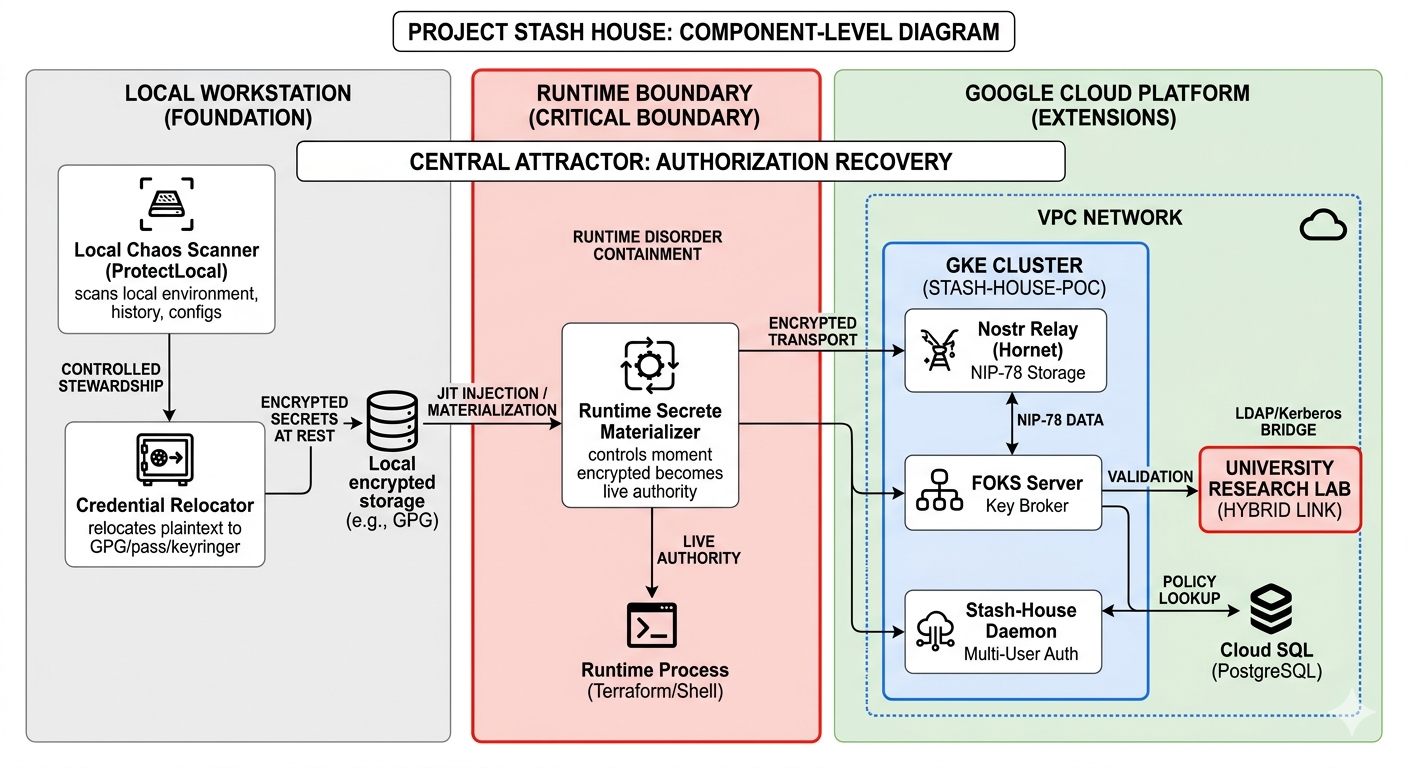
\includegraphics[width=0.4\textwidth]{../../static/images/architecture-component.png}
\end{center}
\end{frame}

{
\usebackgroundtemplate{
\includegraphics[width=\paperwidth]{../../static/images/section.jpg}}
\sectionsubtitle{\textcolor{black}{Securing the Injection Point}}
\section{The Materialization Boundary}
}

\begin{frame}
\frametitle{The Risk of Live Secrets}
\begin{itemize}
\item \textbf{Defining the Boundary:} The precise moment encrypted authority becomes live runtime authority.
\item \textbf{Temporal Exposure:} Minimizing the window between decryption and process consumption.
\item \textbf{JIT Patterns:} Just-in-Time injection into shell environments without disk artifacts.
\end{itemize}
\note[item]{Secrets at rest are easy. Secrets in motion/use are where we fail.}
\end{frame}

{
\usebackgroundtemplate{
\includegraphics[width=\paperwidth]{../../static/images/section.jpg}}
\sectionsubtitle{\textcolor{black}{Sovereign Identity meets Enterprise Governance}}
\section{Federated Infrastructure}
}

\begin{frame}
\frametitle{Nostr Transport \& NIP-78}
\begin{itemize}
\item \textbf{Distributed Redundancy:} Moving from local-only to decentralized event-based storage.
\item \textbf{NIP-78 (Application Data):} Virtual Vaults persisted across relay networks.
\item \textbf{Cryptographic Sovereignty:} Data is signed and encrypted; relays are content-agnostic.
\end{itemize}
\end{frame}

\begin{frame}
\frametitle{FOKS \& Enterprise Bridging}
\begin{itemize}
\item \textbf{FOKS (Federated Open Key Service):} Brokered key release via hardware tokens.
\item \textbf{The Bridge:} Site-to-site tunnels to institutional LDAP and Kerberos servers.
\item \textbf{Mapping Identity:} Projecting sovereign workstation identity into enterprise governance models.
\end{itemize}
\end{frame}

\begin{frame}
\frametitle{Conclusion: Disciplined Identity}
\begin{itemize}
\item \textbf{Recovery > Detection:} Active relocation of authority is the path to hygiene.
\item \textbf{Containment:} Managing the materialization boundary reduces runtime risk.
\item \textbf{Scale:} Decentralized protocols (Nostr/FOKS) enable sovereign security at enterprise scale.
\end{itemize}
\vspace{1em}
\centering
\textbf{Questions?}\\
\small \href{https://github.com/devsecfranklin/stash-house}{github.com/devsecfranklin/stash-house}
\end{frame}

\end{document}